\documentclass[12pt,a4paper,titlepage]{article}
\usepackage{lab_style}
\usepackage{pdfpages}
\usepackage{eso-pic}
\usepackage{graphicx}
\usepackage{float}
\newcommand\tab[1][1cm]{\hspace*{#1}}

\graphicspath{ {images/} }
  
\begin{document}

\begin{titlepage}
\selectlanguage{english}

%----------------------------------------------------------------------------------------
% TITLE PAGE INFORMATION
%----------------------------------------------------------------------------------------
  \begin{center} % Center everything on the page

  %----------------------------------------------------------------------------------------
  % HEADING SECTIONS
  %----------------------------------------------------------------------------------------
  \textsc{\large Faculty of Computers, Informatics and Microelectronics}\\[0.5cm]
  \textsc{\large Technical University of Moldova}\\[1.2cm] % Name of your university/college
  \vspace{25 mm}

  \textsc{\Large Object-Oriented Modeling and Analysis}\\[0.5cm] % Major heading such as course name
  \textsc{\large Laboratory work \#2}\\[0.5cm] % Minor heading such as course title
  %\textsc{\large Laboratory work}\\[0.5cm] % Minor heading such as course title

\newcommand{\HRule}{\rule{\linewidth}{0.5mm}} % Defines a new command for the horizontal lines, change thickness here

  %----------------------------------------------------------------------------------------
  % TITLE SECTION
  %----------------------------------------------------------------------------------------
  \vspace{10 mm}
  \HRule \\[0.4cm]
  { \LARGE \bfseries Use Case Diagrams. Basic and Alternative Flow. Modeling Languages. }\\[0.4cm] % Title of your document
  \HRule \\[1.5cm]

  %----------------------------------------------------------------------------------------
  % AUTHOR SECTION
  %----------------------------------------------------------------------------------------
      \vspace{30mm}

      \begin{minipage}{0.4\textwidth}
      \begin{flushleft} \large
      \emph{Author:}\\
      Cernei \textsc{Liviu}
      \end{flushleft}
      \end{minipage}
      ~
      \begin{minipage}{0.4\textwidth}
      \begin{flushright} \large
      \emph{Supervisor:} \\
      Mihail \textsc{Gavrilița} % Supervisor's Name
      \end{flushright}
      \end{minipage}\\[4cm]

      \vspace{5 mm}
      % If you don't want a supervisor, uncomment the two lines below and remove the section above
      %\Large \emph{Author:}\\
      %John \textsc{Smith}\\[3cm] % Your name

      %----------------------------------------------------------------------------------------
      % DATE SECTION
      %----------------------------------------------------------------------------------------

      %{\large \today}\\[3cm] % Date, change the \today to a set date if you want to be precise

      %----------------------------------------------------------------------------------------
      % LOGO SECTION
      %----------------------------------------------------------------------------------------

      %\includegraphics{red}\\[0.5cm] % Include a department/university logo - this will require the graphicx package

      %----------------------------------------------------------------------------------------

      \vfill % Fill the rest of the page with whitespace
      \end{center}
      
\end{titlepage}

\cleardoublepage

\newpage

\pagenumbering{arabic}
\setcounter{page}{1}
\setcounter{secnumdepth}{4}

\addtocontents{toc}{\protect\thispagestyle{empty}} % no page number on the table of contents page
\cleardoublepage


\phantomsection
\addcontentsline{toc}{section}{Introduction}
\section*{Laboratory work \#2}
\phantomsection

% \section{Purpose of the laboratory}
% Gain knowledge about basics of event-driven programming, understanding of window’s class and basic possibilities of Win32 API. Also she will try to understand and process OS messages.
\section{Tasks}
\begin{itemize}
	\item
	Model your application using 3 Use Case Diagrams;
	\item 
	Create the basic and alternate flows of 3 most important use cases.
\end{itemize}

\section{Theory}
Use case diagrams are used to describe a set of actions (use cases) that some system (subject) can perform in collaboration with one or more external users of the system (actors).

\subsection{Use case diagram elements}
\begin{enumerate}  
	\item Actor - Someone who interacts with use case (system function).
	\item Use Case - System function (process - automated or manual)
	\item Communication Link - a solid link which shows the participation of an actor in a use case 
\end{enumerate}


\subsection{Use Case Relationship}
\begin{enumerate}  

	\item Include
	\begin{enumerate}
		\item When a use case is using functionality of another use case.
		\item An include relationship is depicted with a directed arrow having a dotted line. 
		\item The stereotype "include" identifies the relationship as an include relationship.
	\end{enumerate}
	\item Extends
	\begin{enumerate}  
		\item Whem a use case can be divided in another use cases.
		\item Depicted with a directed arrow having a dotted line. 
		\item The stereotype "extends" identifies as an extend relationship
	\end{enumerate}
	\item Generalization
	\begin{enumerate}  
		\item A generalization relationship is a parent-child relationship between use cases.
		\item The child use case in the generalization relationship can replace the parent use case.
		\item Generalization is shown as a directed arrow with a triangle arrowhead.
	\end{enumerate}
\end{enumerate}

\section{Use Case Diagrams}

\begin{figure}[H]
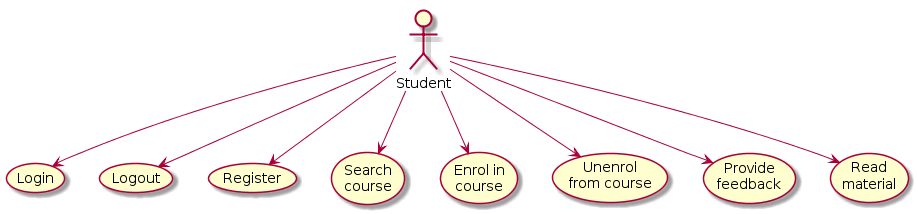
\includegraphics[width=\textwidth]{student}
\caption{Student Use Case diagram}
\centering
\end{figure}

\noindent
Login - to be able to login the student should have an account.\\
Logout - to be able to logout, the student should be logged in.\\
Register - the student must provide personal information (first / last name, year of study, university, faculty. group etc.).\\
Search course - to search a course, the student can input the name of teacher or the title of the course.\\
Enrol in course - the student selects a course, clicks the [Enrol] button and is prompted with a confirmation message.\\
Unenroll from course - the student selects the course clicks the [Unenrol] button and is aked to confirm the operation.\\
Provide feedback - at the bottom of the page is the "Feedback" form with a single field.\\
Read material - the student selects a course in which he is already enroled and can start to read the content.

\clearpage

\begin{figure}[H]
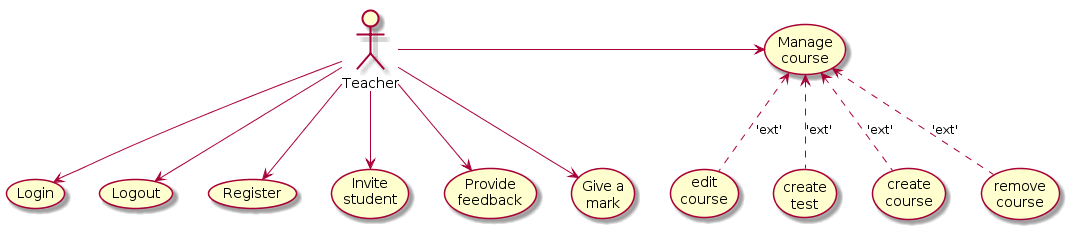
\includegraphics[width=\textwidth]{teacher}
\caption{Teacher Use Case diagram}
\centering
\end{figure}

\noindent
Invite student - the teacher can find a student, invite him to a course which was created by that teacher.\\
Give a mark - the teacher can give a mark to a student enroled in one of his courses.\\
Manage course:\\
\tab Edit course - to edit a course it should be created in advance\\
\tab Create test - at the end of the course, the teacher can append a test.\\
\tab Create course - the teacher must provide a title, date and content (text, images, graphs).\\
\tab Remove course - if the course ended, the teacher can delete it.\\

\clearpage

\begin{figure}[H]
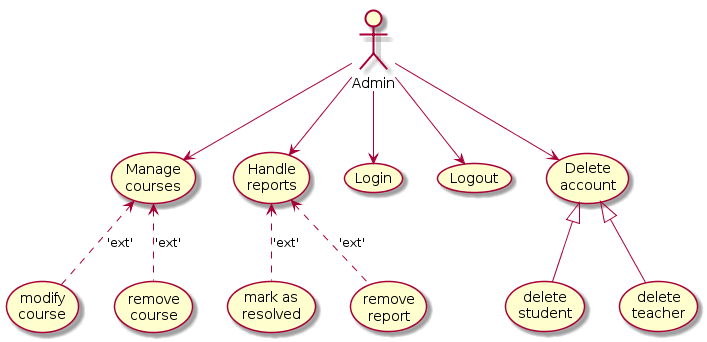
\includegraphics[width=\textwidth]{admin}
\caption{Admin Use Case diagram}
\centering
\end{figure}

\noindent
Handle reports:\\
\tab Mark as resolved - if the feedback of a course has an alert, then it is marked as a report.\\
\tab When the problem is eliminated, the report is resolved.\\
\tab Remove report - if an report is fake or resolved, it can be romoved.\\
Delete account:\\
\tab Delete student - if a person is no longer a student, his account can be removed.
\tab Delete teacher - if a person is no longer a teacher, his account can be removed.

\section{Flow of Events}
\begin{itemize}
\item
\noindent\textbf{Student Use Case diagram - Enrol in course}
\begin{description}
    \item[Success scenario:]
\end{description}
\renewcommand{\labelenumii}{\arabic{enumii}}
\begin{itemize}
  \item 1. The student navigates to "Courses" page
  \item 2. The student selects from the list a course
  \item 3. The student clicks the [Enrol] button.
  \item 4. The system outputs success message.
\end{itemize}
\begin{description}
    \item[Alternate flow:]
\end{description}
\begin{itemize}
  \item 1.a The student enroled to the course by a teacher, other steps are not performed.
  \item 2.a The student inputs name of course in the search box
\end{itemize}

\clearpage

\item
\noindent\textbf{Teacher Use Case diagram - Create course}
\begin{description}
    \item[Success scenario:]
\end{description}
\renewcommand{\labelenumii}{\arabic{enumii}}
\begin{itemize}
  \item 1. The teacher navigates to "Courses" page
  \item 2. The teacher clicks the [New] button.
  \item 3. The teacher writes the title, date, content.
  \item 4. The teacher clicks the [Save] button.
  \item 5. The system outputs success message.
\end{itemize}
\begin{description}
    \item[Alternate flow:]
\end{description}
\begin{itemize}
  \item 3.a The teacher writes the title, date and imports the pdf file with the content.
\end{itemize}

\item
\noindent\textbf{Admin Use Case diagram - Login}
\begin{description}
    \item[Success scenario:]
\end{description}
\renewcommand{\labelenumii}{\arabic{enumii}}
\begin{itemize}
  \item 1. The admin navigates to "Login" page
  \item 2. The admin inputs correct username and correct password.
  \item 3. The admin clicks the [Login] button.
  \item 4. The system outputs success message.
\end{itemize}
\begin{description}
    \item[Alternate flow:]
\end{description}
\begin{itemize}
  \item 2.a The admin inputs wrong username or wrong password, fails to login but attempts one more time with correct username and correct password.
  \item 3.a The admin presses the [Enter] key on the keyboard.

\end{itemize}
\end{itemize}

\clearpage
\cleardoublepage

\end{document}
